\documentclass[svgnames,table,,aspectratio=169]{beamer}
%\documentclass[svgnames,table,handout,aspectratio=129]{beamer}
\usepackage{hhline}
\usepackage{etoolbox}
\usepackage{tikz}
\usepackage{mathtools}
\usepackage{amssymb}
%\usepackage{/usr/lib64/R/share/texmf/Sweave}
\usepackage{polynom}
\usepackage{qrcode}
\usepackage{listings}


%\input{latexdefinitions}
\definecolor{georgiaRed}{RGB}{100,0,00}
\definecolor{mediumGray}{gray}{0.6}



\usetheme{Frankfurt}%
%\usetheme{Warsaw}%
%\useoutertheme{smoothbars}


%\usecolortheme{seagull}
\usecolortheme{beaver}
\logo{\includegraphics[height=.125in]{ugaLogo}}

% Note that the colour definitions are given in the latexDefinitions
% file.
\setbeamercolor{palette primary}{fg=georgiaRed,bg=white}
\setbeamercolor{palette secondary}{fg=georgiaRed,bg=white}
\setbeamercolor{palette tertiary}{fg=georgiaRed,bg=white}
\setbeamercolor{palette quaternary}{bg=mediumGray,fg=black}
\setbeamercolor{block title}{fg=white,bg=georgiaRed}
\setbeamercolor{block body}{fg=black,bg=black!10}
\setbeamercolor{titlelike}{bg=georgiaRed,fg=white} % parent=palette quaternary}

% Define the variable to determine whether or not the clicker quizzes
% are visible in the resulting output.
\newtoggle{clicker}
\toggletrue{clicker}
%\togglefalse{clicker}


% To display a lecture uncomment out the "includeonly" line below to
% match the name of the file. You do not have to do anything with the
% lecture line below and can leave it commented out. It is in place
% because at one time we had multiple lectures within a file, but that
% has been changed.



\mode<presentation>{
  \setbeamercovered{invisible}
  \setbeameroption{hide notes}
}

\mode<handout>{
 
  \usepackage{pgfpages}
  %\pgfpagesuselayout{4 on 1}[letterpaper, border shrink=5mm]
  \pgfpagesuselayout{resize to}[letterpaper,border shrink=5mm]
  \setbeameroption{show notes}


  %\pgfpagesphysicalpageoptions{logical pages=2,physical
  %height=\pgfpageoptionheight,physical width=\pgfpageoptionwidth}
  % Set up the pages for notes.
  % This idea and some code came from
  % http://www.guidodiepen.nl/2009/07/creating-latex-beamer-handouts-with-notes/



  \pgfpagesdeclarelayout{3 on 1 with notes} {
    \edef\pgfpageoptionheight{11in} %\the\paperheight}
    \edef\pgfpageoptionwidth{8.5in} %\the\paperwidth}
    \edef\pgfpageoptionborder{0pt}
  }

  {

	\AtBeginDocument{
      \newbox\notesbox
      \setbox\notesbox=\vbox{
        \hsize=\paperwidth
        \vskip-2.5cm\hskip-5cm\vbox{
          \textcolor{light-gray}{\hrule width 12.6cm\vskip0.5cm}
          \textcolor{light-gray}{\hrule width 12.6cm\vskip0.5cm}
          \textcolor{light-gray}{\hrule width 12.6cm\vskip0.5cm}
          \textcolor{light-gray}{\hrule width 12.6cm\vskip0.5cm}
          \textcolor{light-gray}{\hrule width 12.6cm\vskip0.5cm}
          \textcolor{light-gray}{\hrule width 12.6cm\vskip0.5cm}
          \textcolor{light-gray}{\hrule width 12.6cm\vskip0.5cm}
          \textcolor{light-gray}{\hrule width 12.6cm\vskip0.5cm}
          \textcolor{light-gray}{\hrule width 12.6cm\vskip0.5cm}
          \textcolor{light-gray}{\hrule width 12.6cm\vskip0.5cm}
          \textcolor{light-gray}{\hrule width 12.6cm\vskip0.5cm}
          \textcolor{light-gray}{\hrule width 12.6cm\vskip0.5cm}
          \textcolor{light-gray}{\hrule width 12.6cm\vskip0.5cm}
          \textcolor{light-gray}{\hrule width 12.6cm\vskip0.5cm}
          \textcolor{light-gray}{\hrule width 12.6cm\vskip0.5cm}
          \textcolor{light-gray}{\hrule width 12.6cm\vskip0.5cm}
          \textcolor{light-gray}{\hrule width 12.6cm\vskip0.5cm}
          \textcolor{light-gray}{\hrule width 12.6cm\vskip0.5cm}
          \textcolor{light-gray}{\hrule width 12.6cm\vskip0.5cm}

          \vspace*{-9.75cm}
          \textcolor{light-gray}{\rule[-1.0cm]{1pt}{9.25cm}\hskip0.5cm}
          \textcolor{light-gray}{\rule[-1.0cm]{1pt}{9.25cm}\hskip0.5cm}
          \textcolor{light-gray}{\rule[-1.0cm]{1pt}{9.25cm}\hskip0.5cm}
          \textcolor{light-gray}{\rule[-1.0cm]{1pt}{9.25cm}\hskip0.5cm}
          \textcolor{light-gray}{\rule[-1.0cm]{1pt}{9.25cm}\hskip0.5cm}
          \textcolor{light-gray}{\rule[-1.0cm]{1pt}{9.25cm}\hskip0.5cm}
          \textcolor{light-gray}{\rule[-1.0cm]{1pt}{9.25cm}\hskip0.5cm}
          \textcolor{light-gray}{\rule[-1.0cm]{1pt}{9.25cm}\hskip0.5cm}
          \textcolor{light-gray}{\rule[-1.0cm]{1pt}{9.25cm}\hskip0.5cm}
          \textcolor{light-gray}{\rule[-1.0cm]{1pt}{9.25cm}\hskip0.5cm}
          \textcolor{light-gray}{\rule[-1.0cm]{1pt}{9.25cm}\hskip0.5cm}
          \textcolor{light-gray}{\rule[-1.0cm]{1pt}{9.25cm}\hskip0.5cm}
          \textcolor{light-gray}{\rule[-1.0cm]{1pt}{9.25cm}\hskip0.5cm}
          \textcolor{light-gray}{\rule[-1.0cm]{1pt}{9.25cm}\hskip0.5cm}
          \textcolor{light-gray}{\rule[-1.0cm]{1pt}{9.25cm}\hskip0.5cm}
          \textcolor{light-gray}{\rule[-1.0cm]{1pt}{9.25cm}\hskip0.5cm}
          \textcolor{light-gray}{\rule[-1.0cm]{1pt}{9.25cm}\hskip0.5cm}
          \textcolor{light-gray}{\rule[-1.0cm]{1pt}{9.25cm}\hskip0.5cm}
          \textcolor{light-gray}{\rule[-1.0cm]{1pt}{9.25cm}\hskip0.5cm}
          \textcolor{light-gray}{\rule[-1.0cm]{1pt}{9.25cm}\hskip0.5cm}

        }

      }

    \pgfpagesphysicalpageoptions
    {%
      logical pages=6,%
      physical height=\pgfpageoptionheight,%
      physical width=\pgfpageoptionwidth,%
      last logical shipout=3%
    }
    
    \pgfpageslogicalpageoptions{1}
    {%
      border shrink=\pgfpageoptionborder,%
      resized width=.5\pgfphysicalwidth,%
      resized height=.33\pgfphysicalheight,%
      center=\pgfpoint{.25\pgfphysicalwidth}{.82\pgfphysicalheight}%
    }%
    \pgfpageslogicalpageoptions{2}
    {%
      border shrink=\pgfpageoptionborder,%
      resized width=.5\pgfphysicalwidth,%
      resized height=.33\pgfphysicalheight,%
      center=\pgfpoint{.25\pgfphysicalwidth}{.47\pgfphysicalheight}%
    }%
    \pgfpageslogicalpageoptions{3}
    {%
      border shrink=\pgfpageoptionborder,%
      resized width=.5\pgfphysicalwidth,%
      resized height=.33\pgfphysicalheight,%
      center=\pgfpoint{.25\pgfphysicalwidth}{.17\pgfphysicalheight}%
    }%	
	\pgfpageslogicalpageoptions{4}
    {%
      border shrink=\pgfpageoptionborder,%
      resized width=.5\pgfphysicalwidth,%
      resized height=.33\pgfphysicalheight,%
      center=\pgfpoint{.85\pgfphysicalwidth}{.82\pgfphysicalheight},%
      copy from=4
    }%
    \pgfpageslogicalpageoptions{5}
    {%
      border shrink=\pgfpageoptionborder,%
      resized width=.5\pgfphysicalwidth,%
      resized height=.33\pgfphysicalheight,%
      center=\pgfpoint{.85\pgfphysicalwidth}{.47\pgfphysicalheight},%
      copy from=5
    }%
    \pgfpageslogicalpageoptions{6}
    {%
      border shrink=\pgfpageoptionborder,%
      resized width=.5\pgfphysicalwidth,%
      resized height=.33\pgfphysicalheight,%
      center=\pgfpoint{.85\pgfphysicalwidth}{.17\pgfphysicalheight},%
      copy from=6
    }%
    
      \pgfpagesshipoutlogicalpage{4}\copy\notesbox
      \pgfpagesshipoutlogicalpage{5}\copy\notesbox
      \pgfpagesshipoutlogicalpage{6}\copy\notesbox
    }
  }

  \pgfpagesuselayout{3 on 1 with notes}

}

\setbeamercolor{upper separation line head}{bg=red}
\setbeamercolor{headline}{bg=red}
\setbeamertemplate{headline}
{%
\begin{beamercolorbox}{section in head/foot}
\insertsectionnavigationhorizontal{.75\textwidth}{}{}
\hfill \insertpagenumber /\insertdocumentendpage
\end{beamercolorbox}%
}
\setbeamercolor{section number projected}{bg=red,fg=black}
\setbeamercolor{subsection number projected}{bg=red,fg=black}
%\setbeamercolor{frametitle}{bg=lightgray,fg=black}

\setbeamertemplate{itemize item}{\color{georgiaRed}$\blacklozenge$}
\setbeamertemplate{itemize subitem}{\color{georgiaRed}$\blacktriangleright$}

\newcommand{\dotfield}[2]{%
  \begin{tikzpicture}[y=0.25cm, x=0.25cm,font=\sffamily]
    \foreach \y in {0,...,#2} {
      \foreach \x in {0,...,#1} {
        \draw[fill=georgiaRed,opacity=0.1] (\x,\y)  circle [radius=0.03em];
      }
    }
  \end{tikzpicture}
}

\newcommand{\twoByTwo}[4]{%
  \left[
    \begin{array}{rr}
      #1 & #2 \\
      #3 & #4 \\
    \end{array}
  \right]
}

\newcommand{\threeByThree}[9]{%
  \left[
    \begin{array}{rrr}
      #1 & #2 & #3 \\
      #4 & #5 & #6 \\
      #7 & #8 & #9
    \end{array}
  \right]
}

\newcommand{\columnVector}[1]{%
  \left[
    \begin{array}{r}
    #1                           
    \end{array}
  \right]
}


\begin{document}



\author{\textsc{T. Alli$^{a}$, K. Black$^{a}$}}
\institute{$^a$Department of Mathematics, University of Georgia, GA}
\subject{Linear Algebra}
\keywords{Linear Transformation, Vectors, Matrices, Linear Algebra}

%\lecture{Partial Fractions}{partial-fractions}
%\section{Rational Functions}

\title{Section 6.5: The Method Of Least Squares}
\subtitle{Which Is More Better?}


\date{} % {\today}

\begin{frame}
  \titlepage
\end{frame}

\begin{frame}{Outline}
  \tableofcontents
\end{frame}


\section{Goals}

\begin{frame}{Goals}

  \begin{itemize}
  \item Use the method of  least squares to determine a ``Best Fit''
  \item Convert a data fitting problem to a least squares system.
  \item Determine the residual of a least square solution.
  \end{itemize}

\end{frame}

\begin{frame}{Side Note: Orthogonal Vectors}

  If two vectors, $\vec{u}$ and $\vec{v}$ are orthogonal then
  \begin{eqnarray*}
    \vec{u} \cdot \vec{v} & = & 0.
  \end{eqnarray*}

  Equivalent notation if $\vec{u}$ and $\vec{v}$ are column vectors,
  \begin{eqnarray*}
    \vec{u}^T \vec{v} & = & 0.
  \end{eqnarray*}
  
\end{frame}

\section{Example 2D Problem}

\begin{frame}{Example: The Problem In 2D}

  Suppose we have a linear relationship between two variables:
  \begin{eqnarray*}
    y & = & m_1 x + b.
  \end{eqnarray*}

  We make a large number of observations in an experiment:
  \begin{eqnarray*}
    \begin{array}{r|r}
      x & y \\ \hline
      x_1 & y_1 \\ 
      x_2 & y_2 \\
      x_3 & y_3 \\
      \vdots & \vdots \\
      x_n & y_n
    \end{array}
  \end{eqnarray*}

\end{frame}

\begin{frame}{Look At The Data}

  Now we look at the data to see what we get....

  \begin{center}
    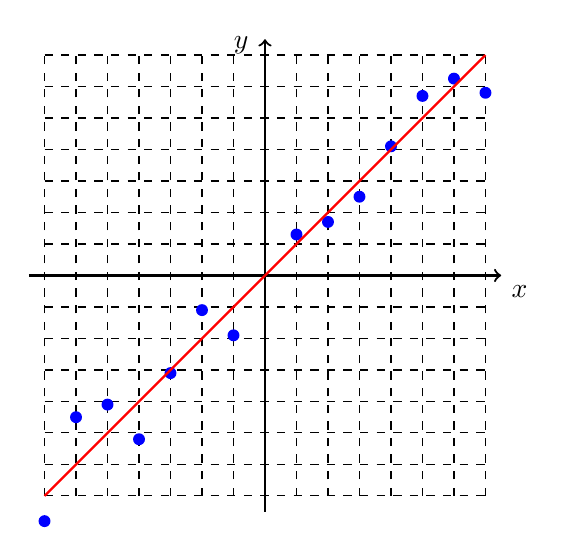
\begin{tikzpicture}[y=0.4cm, x=0.4cm,font=\sffamily]
      %% ticks
      \draw[xstep = 1.0, ystep=1.0,black,dashed,thin] (-7.0, -7.0) grid (7.0, 7.0);

      %% axis
      \draw[thick,->] (-7.5,0) -- coordinate (x axis mid) (7.5,0)
           node[anchor = north west] {$x$};

      \draw[thick,->] (0,-7.5) -- coordinate (y axis mid) (0,7.5)
            node[anchor = east,shift={(-0.2,-0.2)}] {$y$};

      \fill[blue] ( 1, 1.3) circle [radius=0.5ex];
      \fill[blue] ( 2, 1.7) circle [radius=0.5ex];
      \fill[blue] ( 3, 2.5) circle [radius=0.5ex];
      \fill[blue] ( 4, 4.1) circle [radius=0.5ex];
      \fill[blue] ( 5, 5.7) circle [radius=0.5ex];
      \fill[blue] ( 6, 6.25) circle [radius=0.5ex];
      \fill[blue] ( 7, 5.8) circle [radius=0.5ex];
      \fill[blue] (-1,-1.9) circle [radius=0.5ex];
      \fill[blue] (-2,-1.1) circle [radius=0.5ex];
      \fill[blue] (-3,-3.1) circle [radius=0.5ex];
      \fill[blue] (-4,-5.2) circle [radius=0.5ex];
      \fill[blue] (-5,-4.1) circle [radius=0.5ex];
      \fill[blue] (-6,-4.5) circle [radius=0.5ex];
      \fill[blue] (-7,-7.8) circle [radius=0.5ex];

      \uncover<2->{\draw[red,thick] (-7,-7) -- (7,7);}

    \end{tikzpicture}
  \end{center}
  
\end{frame}

\begin{frame}{How Do We Approximate $m$ and $b$?}
 
  We started with
  \begin{eqnarray*}
    y & = & m_1 x + b,
  \end{eqnarray*}
  but now there are many equations And two unknowns.

  It is not consistent, so how do we decide what values to use for
  $m_1$ and $b$????

  \vfill
  
\end{frame}

\begin{frame}{Define The System}

  \begin{columns}
    \column{0.5\textwidth}
    First, define the system,
    \begin{eqnarray*}
      m_1 x_1 + b & \approx & y_1, \\
      m_1 x_2 + b & \approx & y_2, \\
      m_1 x_3 + b & \approx & y_3, \\
      \vdots & & \vdots \\
      m_1 x_n + b & \approx & y_n, \\
    \end{eqnarray*}

    \column{0.5\textwidth}
    In matrix form:
    \begin{eqnarray*}
      \left[
      \begin{array}{rr}
        x_1 & 1 \\
        x_2 & 1 \\
        x_3 & 1 \\
        \vdots & \vdots \\
        x_n & 1
      \end{array}
              \right]
              \columnVector{m_1 \\ b}
            & \approx &
                  \columnVector{y_1 \\ y_2 \\ y_3 \\ \vdots \\ y_n}.
    \end{eqnarray*}
  \end{columns}
\end{frame}


\section{The Residual}

\begin{frame}{Define The Residual}

  The system is in the form
  \begin{eqnarray*}
    A \vec{x} & \approx & \vec{b}.
  \end{eqnarray*}
  It is not exact, though.

  So we define the residual
  \begin{eqnarray*}
    \vec{r} & = & A \vec{x} - \vec{b}.
  \end{eqnarray*}

  The residual is not the zero vector, but we want it to be as close
  as possible.
  
\end{frame}

\begin{frame}{How To Pick $\vec{x}$?}

  \only<1>{
    \begin{itemize}
    \item $A\vec{x}$, is a linear combination of the columns of $A$.
    \item $\vec{b}$ is likely not in the column space of $A$.
    \item Choose a vector $\vec{x}$ so that the residual is
      orthogonal to the column space of $A$.
    \end{itemize}

    \vfill
  }

  \begin{center}
    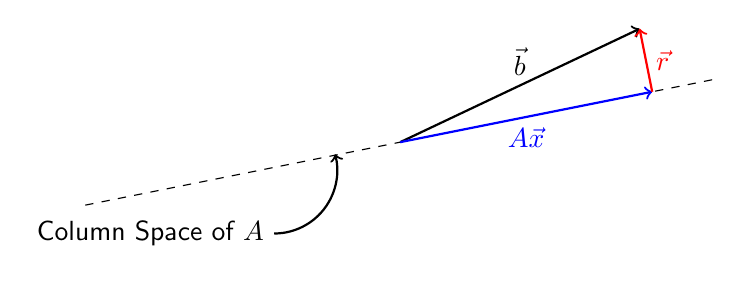
\begin{tikzpicture}[y=0.8cm, x=0.8cm,font=\sffamily]
      %% ticks

      \draw[thin,black,dashed] (-5,-1) -- (5,1);
      \draw[thick,black,->]  (0,0) -- (3.8,1.8) node [pos=0.5,above] {$\vec{b}$};
      \draw[thick,blue,->] (0,0) -- (4,0.8) node [pos=0.5,below] {$A\vec{x}$};
      \draw[thick,red,->]  (4,0.8) -- (3.8,1.8) node [pos=0.5,right] {$\vec{r}$};
      \draw[thick,black,->] (-2,-1.45) arc(270:375:1) node [pos=0,left] {Column Space of $A$};

    \end{tikzpicture}
  \end{center}

  \begin{eqnarray*}
    \only<2->{\vec{a}_1^T\vec{r}} & \only<2->{=} & \only<2->{0} \\
    \only<3->{\vec{a}_2^T\vec{r}} & \only<3->{=} & \only<3->{0} \\
    \only<4->{\vec{a}_3^T\vec{r}} & \only<4->{=} & \only<4->{0} \\
    \only<5->{\vdots} & &  \\
    \only<5->{\vec{a}_n^T\vec{r}} & \only<5->{=} & \only<5->{0} \\
  \end{eqnarray*}
  
\end{frame}

\section{Least Squares Approximation}

\begin{frame}{Matrix Equation}

  This is equivalent to first defining the residual
  \begin{eqnarray*}
    \vec{r} & = & A\vec{x} - \vec{b}.
  \end{eqnarray*}

  Now require that the residual be orthogonal to the column space
  \begin{eqnarray*}
    A^T \vec{r} & = & \vec{0}, \\
    A^T \left( A \vec{x} - \vec{b} \right) & = & \vec{0}.
  \end{eqnarray*}

  Multiply the $A^T$ through, and solve for $\vec{x}$.
  
\end{frame}

\section{Examples}

\begin{frame}{Example One}

  Suppose we have
  \begin{eqnarray*}
    y & = & m_1 x + b,
  \end{eqnarray*}
  
  \begin{columns}
    \column{0.5\textwidth}
    And we have the following measurements:
    \begin{eqnarray*}
      \begin{array}{r|r}
        x & y \\ \hline
        1 & 3.1 \\
        1 & 3.2 \\
        2 & 3.8 \\
        2 & 4.1 \\
        3 & 5.2 \\
        3 & 5.3 \\
      \end{array}
    \end{eqnarray*}

    \column{0.5\textwidth}

    \begin{eqnarray*}
      m_1 1 + b & \approx & 3.1 \\
      m_1 1 + b & \approx & 3.2 \\
      m_1 2 + b & \approx & 3.8 \\
      m_1 2 + b & \approx & 4.1 \\
      m_1 3 + b & \approx & 5.2 \\
      m_1 3 + b & \approx & 5.3 \\
    \end{eqnarray*}

    
  \end{columns}
\end{frame}

\begin{frame}{Example One}

    \begin{center}
    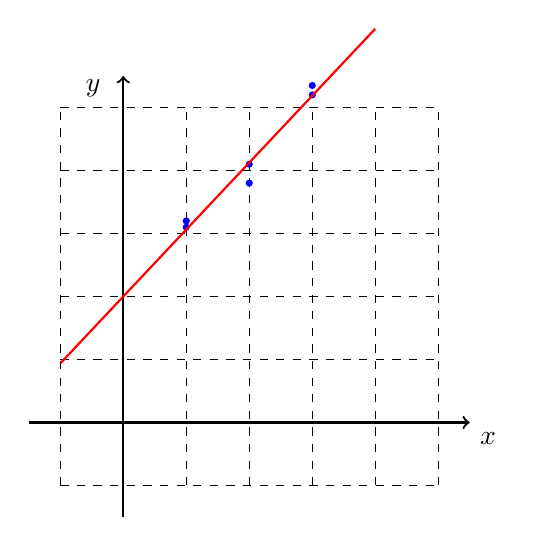
\begin{tikzpicture}[y=0.8cm, x=0.8cm,font=\sffamily]
      %% ticks
      \draw[xstep = 1.0, ystep=1.0,black,dashed,thin] (-1.0, -1.0) grid (5.0, 5.0);

      %% axis
      \draw[thick,->] (-1.5,0) -- coordinate (x axis mid) (5.5,0)
           node[anchor = north west] {$x$};

      \draw[thick,->] (0,-1.5) -- coordinate (y axis mid) (0,5.5)
            node[anchor = east,shift={(-0.2,-0.2)}] {$y$};

      \fill[blue] ( 1, 3.1) circle [radius=0.3ex];
      \fill[blue] ( 1, 3.2) circle [radius=0.3ex];
      \fill[blue] ( 2, 3.8) circle [radius=0.3ex];
      \fill[blue] ( 2, 4.1) circle [radius=0.3ex];
      \fill[blue] ( 3, 5.2) circle [radius=0.3ex];
      \fill[blue] ( 3, 5.35) circle [radius=0.3ex];

      \uncover<2->{\draw[red,thick] (-1,0.9375) -- (4,6.25);}

    \end{tikzpicture}

%> x <- c(1,1,2,2,3,3)
%> y <- c(3.1,3.2,3.8,4.1,5.2,5.35)
%> l <- lm(y~x)
%> l
%
%Call:
%lm(formula = y ~ x)
%
%Coefficients:
%(Intercept)            x  
%      2.000        1.062  
%
%> l$
%l$coefficients   l$rank           l$qr             l$call           
%l$residuals      l$fitted.values  l$df.residual    l$terms          
%l$effects        l$assign         l$xlevels        l$model          
%> l$coefficients
%(Intercept)           x 
%     2.0000      1.0625 
%> l$coefficients[[1]]
%[1] 2
%> l$coefficients[[2]]
%[1] 1.0625
%> l$coefficients[[2]]*-1+l$coefficients[[1]]
%[1] 0.9375
%> l$coefficients[[2]]*4+l$coefficients[[1]]
%[1] 6.25
%> 

  \end{center}

\end{frame}

\begin{frame}{Example One}

  \begin{columns}
    \column{0.5\textwidth}

    \begin{eqnarray*}
      m_1 1 + b & \approx & 3.1 \\
      m_1 1 + b & \approx & 3.2 \\
      m_1 2 + b & \approx & 3.8 \\
      m_1 2 + b & \approx & 4.1 \\
      m_1 3 + b & \approx & 5.2 \\
      m_1 3 + b & \approx & 5.3 \\
    \end{eqnarray*}

    \column{0.5\textwidth}

    \begin{eqnarray*}
      \vec{r} & = & 
      \left[
      \begin{array}{rr}
        1 & 1 \\
        1 & 1 \\
        2 & 1 \\
        2 & 1 \\
        3 & 1 \\
        3 & 1 \\
      \end{array}
      \right]
      \columnVector{m_1 \\ b} - 
      \columnVector{3.1 \\ 3.2 \\ 3.8 \\ 4.1 \\ 5.2 \\ 5.3}
  \end{eqnarray*}

    
  \end{columns}
\end{frame}



\begin{frame}{Example One}

  \begin{eqnarray*}
    A^T \left( A \vec{x} - \vec{b} \right) & = & \vec{0}, \\
    A^T A \vec{x} - A^T \vec{b}  & = & \vec{0}, \\
    A^T A \vec{x}  & = & A^T \vec{b}, \\
  \end{eqnarray*}

  \only<1>{
  \begin{eqnarray*}
    \left[
      \begin{array}{rrrrrr}
        1 & 1 & 2 & 2 & 3 & 3\\
        1 & 1 & 1 & 1 & 1 & 1 
      \end{array}
      \right]
    \left[
    \begin{array}{rr}
       1 & 1 \\
       1 & 1 \\
       2 & 1 \\
       2 & 1 \\
       3 & 1 \\
       3 & 1 \\
    \end{array}
    \right]
    \columnVector{m_1 \\ b}
    & = &
    \left[
      \begin{array}{rrrrrr}
        1 & 1 & 2 & 2 & 3 & 3\\
        1 & 1 & 1 & 1 & 1 & 1 
      \end{array}
      \right]
    \columnVector{3.1 \\ 3.2 \\ 3.8 \\ 4.1 \\ 5.2 \\ 5.3}
  \end{eqnarray*}
  }

  \only<2>{
  \begin{eqnarray*}
    \left[
    \begin{array}{rr}
      28 & 12 \\
      12 & 6
    \end{array}
    \right]
    \columnVector{m_1 \\ b}
         & = &
               \columnVector{53.6 \\ 24.7}
  \end{eqnarray*}
}


\end{frame}

\begin{frame}[fragile]{MATLAB Code}
  \lstset{basicstyle=\tiny\ttfamily,breaklines=true}
  \lstset{framextopmargin=50pt,frame=bottomline}

  \begin{columns}
    \column{0.5\textwidth}

    \begin{lstlisting}
A = [1 1; 1 1; 2 1 ;  2 1; 3 1 ; 3 1]
A =

   1   1
   1   1
   2   1
   2   1
   3   1
   3   1

> b = [3.1 ; 3.2 ; 3.8 ; 4.1 ;5.2 ; 5.3]
b =

   3.1000
   3.2000
   3.8000
   4.1000
   5.2000
   5.3000

\end{lstlisting}

\column{0.5\textwidth}

\begin{lstlisting}
> LSQ = A'*A
LSQ =

   28   12
   12    6

> rightSide = A'*b
rightSide =

   53.600
   24.700

> x = LSQ\rightSide 
x =

   1.0500
   2.0167

\end{lstlisting}

  \end{columns}
\end{frame}

\begin{frame}{Example Two}

  Suppose we have
  \begin{eqnarray*}
    \left[
    \begin{array}{rrr}
      -3 & -3 & 1 \\
      -3 & -2 & 1 \\
      -2 & -2 & 1 \\
      -2 & -1 & 1 \\
      -1 & -1 & 1 \\
      -1 &  0 & 1 \\
       0 &  0 & 1 \\
       0 &  1 & 1 \\
       1 &  1 & 1 \\
       1 &  2 & 1 \\
       2 &  2 & 1 \\
       2 &  3 & 1 \\
       3 &  3 & 1 \\
       3 &  4 & 1 \\
    \end{array}
    \right]
    \columnVector{m_1 \\ m_2 \\ b}
    & \approx &
    \columnVector{2.54 \\ 2.26 \\ 3.49 \\ 2.05 \\ 1.66 \\ 2.47 \\ 4.08 \\
                  1.66 \\ 2.89 \\ 2.75 \\ 2.55 \\ 1.03 \\ 1.90 \\ 1.98 }
  \end{eqnarray*}
  
\end{frame}


\begin{frame}{Example Two}

  Define the matrix and vector:
  \begin{columns}
    \column{0.5\textwidth}
  \begin{eqnarray*}
    A & = & 
    \left[
    \begin{array}{rrr}
      -3 & -3 & 1 \\
      -3 & -2 & 1 \\
      -2 & -2 & 1 \\
      -2 & -1 & 1 \\
      -1 & -1 & 1 \\
      -1 &  0 & 1 \\
       0 &  0 & 1 \\
       0 &  1 & 1 \\
       1 &  1 & 1 \\
       1 &  2 & 1 \\
       2 &  2 & 1 \\
       2 &  3 & 1 \\
       3 &  3 & 1 \\
       3 &  4 & 1 \\
    \end{array}
    \right]
  \end{eqnarray*}

  \column{0.5\textwidth}
  \begin{eqnarray*}
    \vec{b} & = &  \columnVector{2.54 \\ 2.26 \\ 3.49 \\ 2.05 \\ 1.66 \\ 2.47 \\ 4.08 \\
                  1.66 \\ 2.89 \\ 2.75 \\ 2.55 \\ 1.03 \\ 1.90 \\ 1.98 }
  \end{eqnarray*}

\end{columns}
\end{frame}


\begin{frame}{Example Two}

  \begin{eqnarray*}
    A^TA \vec{x} & = & A^T\vec{b}, \\
    \left[
    \begin{array}{rrr}
      56 & 56 & 0 \\
      56 & 63 & 7 \\
      0 & 7 & 14
    \end{array}
    \right]
    \vec{x} & = & \columnVector{-5.17 \\ 9.03 \\ 33.31}
  \end{eqnarray*}

  Solving we get
  \begin{eqnarray*}
    \columnVector{m_1 \\ m_2 \\ b} & \approx & \columnVector{ 0.609 \\ -0.701 \\ 2.73 }
  \end{eqnarray*}
  
\end{frame}

\begin{frame}{Note: Symmetric Matrix}

  We are solving a system of the form
  \begin{eqnarray*}
    A^TA\vec{x} & = & A^T\vec{b}.
  \end{eqnarray*}
  The matrix $A^TA$ is symmetric!

  In practice $A^TA$ is ill-conditioned, and we do not solve it using
  row reduction, instead we use QR decomposition,
  \begin{eqnarray*}
    A^TA & = & QR.
  \end{eqnarray*}
  
\end{frame}

\begin{frame}{Blank Page}
  \dotfield{60}{24}
\end{frame}


\end{document}

  We have a linear relationship between variables:
  \begin{eqnarray*}
    y & = & m_1 x_1 + m_2 x_2 + \cdots + m_l x_l.
  \end{eqnarray*}

  Suppose we make large number of observations in an experiment:
      \begin{eqnarray*}
      \begin{array}{lr|r|r|r|r|r}
        \mathrm{Experiment~1}: & x_{11}  & x_{21} & x_{31} & \ldots & x_{l1} & z_1 \\
        \mathrm{Experiment~2}: & x_{12}  & x_{22} & x_{32} & \ldots & x_{l2} & z_2 \\
        \mathrm{Experiment~3}: & x_{13}  & x_{23} & x_{33} & \ldots & x_{l3} & z_3 \\
        \vdots & \vdots & \vdots & \vdots & \vdots & \vdots \\
        \mathrm{Experiment~n}: & x_{1n}  & x_{2n} & x_{3n} & \ldots & x_{l1} & z_n 
      \end{array}
      \end{eqnarray*}
